% !TEX root = cha-application.tex
\documentclass[../../main.tex]{subfiles}

\begin{document}

\section{Impact of Path Boost}
\label{sec:path_boost_effect}
This experiment evaluates the effect of path boost on generating valid solutions. We used the complete class hierarchy of the Pharo \texttt{Slot} class, which contains 30 classes.

We ran 48 instances over a period of four days. Half of the instances were run without path boost, while the other half used a path boost of 50. All other configuration parameters were kept the same. For both configurations, the 24 instances were divided into three groups of 8, with a minimum class distance of 1, 2, and 3.

The results are summarized in \tabref{tab:path_boost_results}. Without path boost, no valid solution was found in any of the 24 instances. WFC performed a total of 2,332,200 attempts: 804,250 with distance 1, 808,700 with distance 2, and 719,250 with distance 3. Despite the large number of attempts, none produced a valid solution.

\begin{table}[ht]
    \centering
    \rowcolors{3}{xcolorblue}{white}
    \begin{tabular}{c|c|c|c|c}
        \textbf{Path Boost} & \textbf{Min Distance} & \textbf{Instances} & \textbf{Solutions} & \textbf{Success Rate} \\
        \hline
        No & 1 & 8 & 0 & 0\% (0/8) \\
        No & 2 & 8 & 0 & 0\% (0/8) \\
        No & 3 & 8 & 0 & 0\% (0/8) \\
        \hline
        50 & 1 & 8 & 1 & 12.5\% (1/8) \\
        50 & 2 & 8 & 4 & 50.0\% (4/8) \\
        50 & 3 & 8 & 2 & 25.0\% (2/8) \\
    \end{tabular}
    \caption{Results obtained with and without path boost, for each minimum class distance.}
    \label{tab:path_boost_results}
\end{table}

Without path boost, paths are not guided toward their target classes. The fixed exit directions only give them an initial direction, after which they are generated completely randomly based on the weighted choice. Therefore, the paths must reach their targets by chance. When many paths are generated at the same time, it is very unlikely that all of them will meet the correct targets.

With path boost enabled, 6 valid solutions were found. For distance 1, one solution was found after 23 hours, 42 minutes, and 44 seconds. For distance 2, four solutions were found after 37.43 seconds, 32 minutes and 47 seconds, 10 hours, 25 minutes and 30 seconds, and 18 hours and 14 minutes. For distance 3, two solutions were found after 35 minutes and 36 seconds, and 1 hour, 14 minutes and 33 seconds. Execution times are shown in \figref{fig:path_boost_execution_times}.

\begin{figure}[ht]
    \centering
    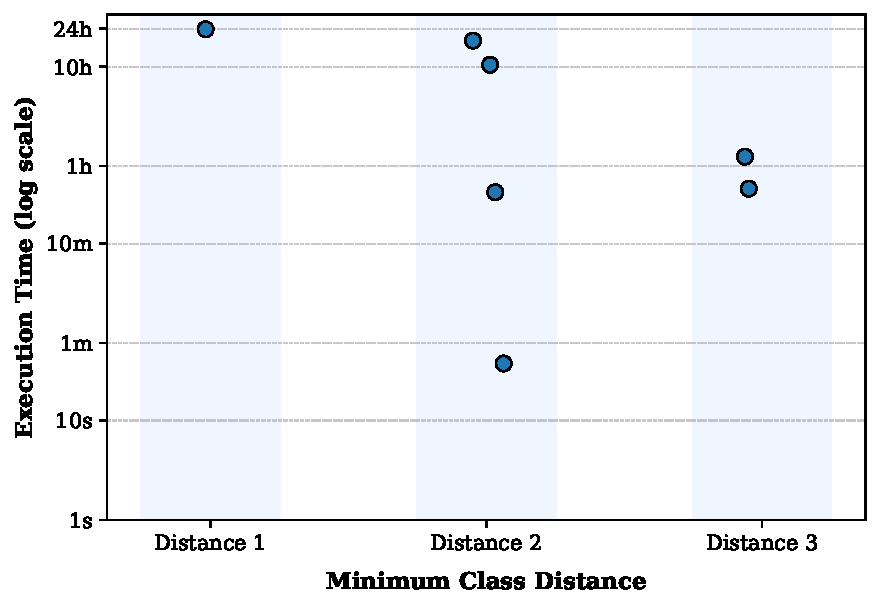
\includegraphics[width=0.85\linewidth]{figures/application/path_boost_execution_times}
    \caption{Execution times grouped by minimum class distance (with path boost).}
    \label{fig:path_boost_execution_times}
\end{figure}

The comparison shows that path boost has a strong effect on the ability of WFC to find valid solutions. It is also interesting to note that after 1 day no other solutions were found, suggesting that when the grid becomes too large it becomes more difficult for WFC to find a valid solution. This may be correlated with what was shown in \secref{sec:min_distance_comparison}.

\figref{fig:slot_path_boost} shows the solution found after 37.43 seconds with a minimum class distance of 2.

\begin{figure}[ht]
    \centering
    \includegraphics[width=0.7\textwidth]{figures/application/slot_path_boost}
    \caption{\texttt{Slot} hierarchy generated with path boost 50 and minimum distance 2 (37.34s).}
    \label{fig:slot_path_boost}
\end{figure}

\end{document}